\documentclass[
hyperref={pdfpagelabels=false}
%,red %, notes=show
,xcolor=table
% ,handout % UNCOMMENT FOR HANDOUT - also uncomment \pgfpagesuselayout
]
{beamer}

%\usecolortheme{beaver}


\setlength {\marginparwidth }{2cm}
\usepackage{todonotes}

\definecolor{Myred}{rgb}{0.7, 0.2, 0.2}

\usecolortheme[named=Myred]{structure}



\newcommand{\plus}{{
\includegraphics[scale=0.01]{plus.png}}}
\newcommand{\minus}{{
\includegraphics[scale=0.06]{minus.png}}}

\usepackage{bm}


\usepackage{pres}
% \usepackage{mathdots}
%\usepackage{qtree}
\usepackage{pgfpages}
% \pgfpagesuselayout{4 on 1}[a4paper, landscape,border shrink=5mm]
%\pgfpagesuselayout{2 on 1}[a4paper,border shrink=5mm]
\pgfpageslogicalpageoptions{1}{border code=\pgfusepath{stroke}}
\pgfpageslogicalpageoptions{2}{border code=\pgfusepath{stroke}}
\pgfpageslogicalpageoptions{3}{border code=\pgfusepath{stroke}}
\pgfpageslogicalpageoptions{4}{border code=\pgfusepath{stroke}}

\usepackage{picture}
\usepackage{pgfplots}
% \usepackage{filecontents}
% \pgfplotsset{compat=1.12}
\usepackage{pdflscape}

\beamertemplatenavigationsymbolsempty

\newcommand{\travail}{\textbf{ICI IL Y A D TRAVAIL!}}

\usepackage{listings}
\makeatletter
\lstset{
  language={C},
  frame=single,
  basicstyle=\lst@ifdisplaystyle\tiny\fi\ttfamily,
  columns=fullflexible,
  keepspaces=true,
  keywordstyle=\color{blue}
}

\usepackage{pdfcomment}
\newcommand{\pdfnote}[1]{\marginnote{\pdfcomment[icon=note]{#1}}}


\newcommand\Wider[2][5em]{%
\makebox[\linewidth][c]{%
  \begin{minipage}{\dimexpr\textwidth+#1\relax}
  \raggedright#2
  \end{minipage}%
  }%
}


\AtBeginSection[]{
    \begin{frame}
    \vfill
    \centering
    \begin{beamercolorbox}[sep=8pt,center,shadow=true,rounded=true]{section page}
        \usebeamerfont{title}%
        {\Huge \insertsectionhead}\par
    \end{beamercolorbox}
    \vfill
    \end{frame}
}




%%%%%%%%%%%%%%%%%%%%%%%%%%%%%
%%%%% PRESENTATION INFO %%%%%
%%%%%%%%%%%%%%%%%%%%%%%%%%%%%
\title[CSC - Intro]{Introduction \\ -- Cryptography and Secured Communications --} 
\author[]{Lionel Morel}
\institute[]{Telecommunications - INSA Lyon}
\date{Fall-Winter 2022-23}


%%%%%%%%%%%%%%%%%%%%%%%%%
%%%%%%%% COLORS %%%%%%%%%
%%%%%%%%%%%%%%%%%%%%%%%%%
\definecolor{greenCiti}{RGB}{83,186,89}
\definecolor{darkGreen}{RGB}{60,132,136}
\definecolor{purple}{RGB}{76, 69, 164}
\colorlet{corecolor}{lightgray}
\definecolor{uncorecolor}{RGB}{222,181,182}
\definecolor{lightgray}{rgb}{0.8,0.8,0.8}
\definecolor{lightblue}{RGB}{188,212,244}
\colorlet{socketcolor}{blue!20}

\colorlet{getpcolor}{red}
\colorlet{leetcolor}{darkGreen}

\definecolor{redfixit}{RGB}{188,43,0}
\definecolor{yellowfixit}{RGB}{235,237,62}
\definecolor{bluefixit}{RGB}{7,2,236}
\definecolor{orangefixit}{RGB}{227,118,24}
\definecolor{cyanfixit}{RGB}{1,171,159}
\definecolor{purplefixit}{RGB}{206,92,232}
\definecolor{greenfixit}{RGB}{102,156,52}



\begin{document}

\begin{frame}
  \maketitle
\end{frame}

% \begin{frame}[fragile]
%   \frametitle{A FAIRE AVANT LE PREMIER COURS}

%   \begin{itemize}
%   \item \textbf{Vérifier} que tous les TODOs sont traités
%   \item Préparer des notes autour des slides pour :
%     \begin{itemize}
%     \item les anecdotes
%     \item le choix de l'ordre des description de certains exemples
%     \end{itemize}
%   \item Ajouter des ``justifications'' au topics:
%     \begin{itemize}
%     \item on veut lever le voile sur https,
%     \item On veut vous faire comprendre que la sécurité c'est bcp
%       d'aspects différents: la sécurité des communication
%       (chiffrement), la sécurité des infos de crypto (comment on
%       génère des clefs et comment on les protège), la sécurité physique. 
%     \end{itemize}
%   \item est-ce que je saurais dessiner un panorama des types
%     d'attaques (à très gros traits). Par exemple en donnant des
%     exemples des différents types, piochés là :
%     \url{https://en.wikipedia.org/wiki/Computer_security#Vulnerabilities_and_attacks}
%   \item Au delà, donner des ``attaques récentes'', par exemple tirées de là :
%    \url{https://www.schneier.com/}
%   \end{itemize}
% \end{frame}



\section{Introduction}

\begin{frame}
  \frametitle{Lecturer - Lionel Morel (lionel.morel@insa-lyon.fr)}
  \Wider{\begin{itemize}
  \item MSc in Computer Science - Grenoble 2001
  \item PhD in CS at INPGrenoble - Programming of Critical Reactive Systems
  \item Associate Professor at INSA Lyon since 2007. 
  \item (past) Research topics:
    \begin{itemize}
    \item at Grenoble, Turku (Finland), Rennes, and Lyon: Models of
      concurrency and computations, programming languages, performance
      analysis for parallel multi-core architectures.
    \item at CEA-Grenoble (2017-2020): \textbf{Counter-measures
        against physical  attacks (side-channel, fault-injection, etc)}
    \end{itemize}
  \item Current Research: \textbf{operating systems} and programming
    languages \textbf{for} addressing so-called \textbf{frugality}, Phenix \footnote{\url{https://phenix.citi-lab.fr/}, \url{lionel.morel.ouvaton.org}}
  \item Teaching at the IF department: Computer Architecture,
    Operating Systems, Compiler Construction
  \end{itemize}
  }
\end{frame}


\begin{frame}
  \frametitle{Un petit détour}

\end{frame}



\section{Course Objectives}



\begin{frame}
  \frametitle{Course Objectives}
  Give you some ``necessary and sufficient'' background on:
  \begin{itemize}
  \item Cryptography
  \item Cryptographic protocols
  \item Public-key infrastructures
  \item Associated ethical issues
  \end{itemize}

  But:
  \begin{itemize}
  \item Security is a vast topic, covered by \textbf{several years} of
    studies if you want to specialize
  \item You will not be a specialist, but a \textbf{enlightened neophytes}. 
  \item[$\Rightarrow$]
  \item Please don't change cryptography yourself
  \item \textbf{Go and ask} a specialist
  \end{itemize}
\end{frame}

\begin{frame}
  \frametitle{Course Plan}

  \Wider{\begin{center}
    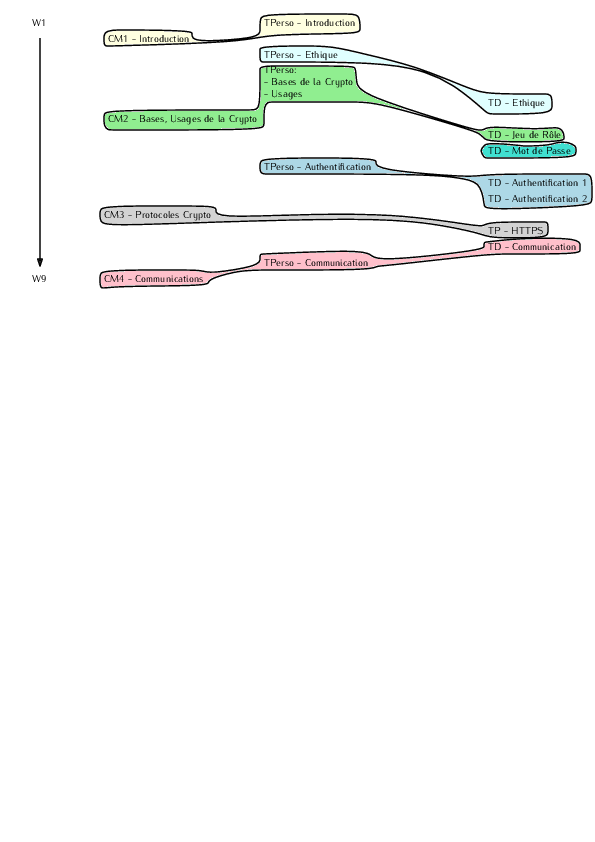
\includegraphics[width=\textwidth,keepaspectratio]{fig/CoursePlan.pdf}
  \end{center}}
\end{frame}

\section{General Considerations}


\begin{frame}
  \frametitle{Information Security}

  \begin{itemize}
  \item \textbf{Information security} $\triangleq$ practice of
    protecting information by mitigating information
    risks\footnote{\url{https://en.wikipedia.org/wiki/Information_security}}
  \item Need to protect all elements dealing with information: computers, networks, people
  \item Security covers a lot of different aspects:  physical security, social engineering, communication security, etc. 
  \item $\triangleq$ practice that allows to maintain the CIA triad (see next)
  \end{itemize}
\end{frame}


\begin{frame}
  \frametitle{The CIA Triad}
  \begin{itemize}
  \item \textbf{Confidentiality}: Information is not made available or
    disclosed to unauthorized individuals, entities, or
    processes.\footnote{\tiny Beckers, K. (2015). Pattern and Security
      Requirements: Engineering-Based Establishment of Security
      Standards.}
  \item \textbf{Integrity}: Information is not modified in an unauthorized or
    undetected manner. Also called \textbf{anti-tampering}.
  \item \textbf{Availability}: Information is available when it is needed.
  \end{itemize}

  \begin{center}
    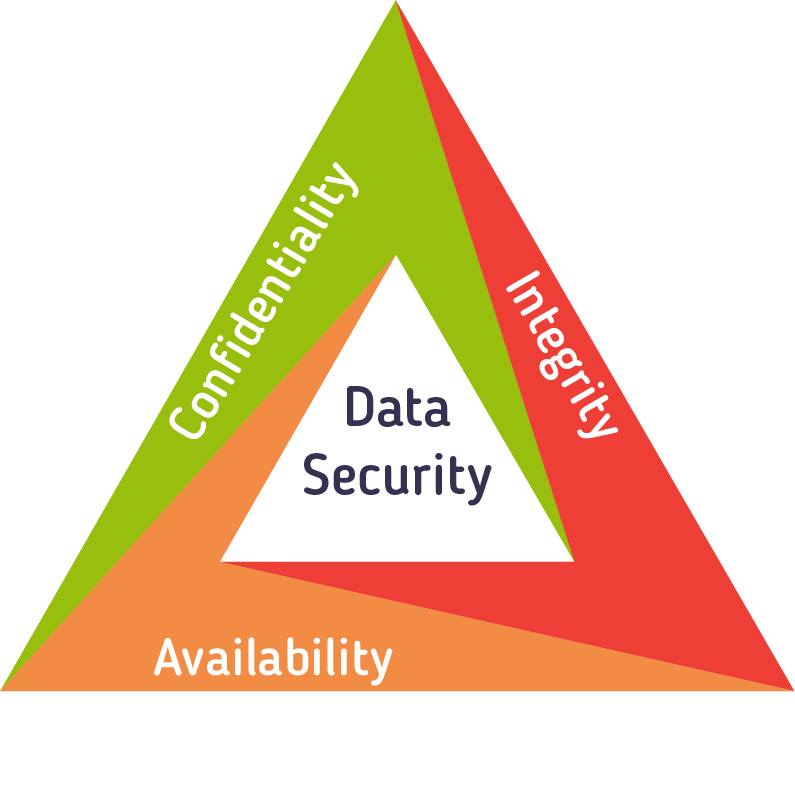
\includegraphics[scale=0.15]{CIA.png}
  \end{center}
  
\end{frame}


\begin{frame}
  \frametitle{Threats}
  \begin{itemize}
  \item A \textbf{threat} is a potential negative action or event that can
    result in unwanted impact to a computer system, application or
    user information.
  \item A \textbf{threat model} is a set of properties that characterize
    threats associated to a particular environment. Often implies
    \textbf{security requirements} on a system. 
  \end{itemize}
\end{frame}


\begin{frame}
  \frametitle{Vulnerabilities}
  \begin{itemize}
  \item A \textbf{vulnerability} is a weakness which can be exploited by an
    attacker to access unauthorized information or to compromise the
    attacked system's behavior. 
  \item The \textbf{attack surface} of a system/application is the set of
    (known) vulnerabilities exposed by it to a potential attacker.
  \end{itemize}
\end{frame}


\begin{frame}
  \frametitle{Attacks}
  \begin{itemize}
  \item \textbf{Attack} = Attempt to exploit a vulnerability
  \item Attack can be:
    \begin{itemize}
    \item Passive (eavesdropping, side-channel, etc)
    \item Active (worm, faults, etc)
    \item Denial-of-service, ie render the service unusable. 
    \end{itemize}
  \item When the attack is successful, we say the system is \textbf{compromised} 
  \end{itemize}
\end{frame}


\begin{frame}
  \frametitle{Trust}
  \begin{itemize}
  \item \textbf{Trust} = Degree to which an entity (person, system, hardware, software) is going to behave as expected
  \item A \textbf{Trust model} describes which entity(ies) is/are
    trusted and at which level.
  \end{itemize}
\end{frame}

\section{The Attacker's Toolbox}


\begin{frame}[fragile]
  \frametitle{Attack Examples}
  \begin{itemize}
  \item \textbf{Trojan}: a malevolent binary that pretends to be something else
  \item \textbf{Worm}: self-replicates to propagate to other computer hosts
  \item \textbf{Virus}: replicates itself by modifying other programs to insert its own code
  \item \textbf{Buffer Overflow}: use adjacent placement of data in memory to modify some private data by writing to public data:
    \begin{center}
      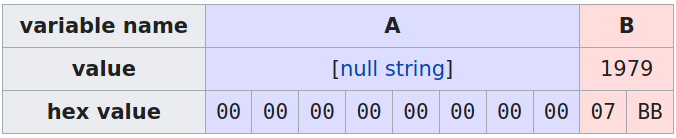
\includegraphics[scale=0.3]{bufferOverflow-init.png}
\begin{verbatim}
char           A[8] = "";
unsigned short B    = 1979;
...
strcpy(A, "excessive");
\end{verbatim}
      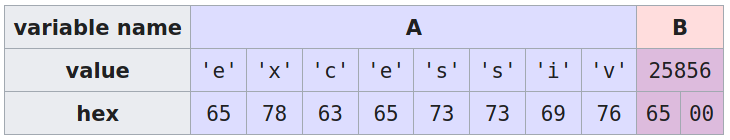
\includegraphics[scale=0.3]{bufferOverflow-final.png}
    \end{center}
  %\item Spoofing, Man-in-the-Middle Attack, Replay
  \end{itemize}
\end{frame}


\begin{frame}[fragile]
  \frametitle{Buffer Overflow}

  $\triangleq$ ``Anomaly whereby a program, while writing data to a buffer,
  overruns the buffer's boundary and overwrites adjacent memory
  locations.''\footnote{\url{https://en.wikipedia.org/wiki/Buffer_overflow}}

  \begin{itemize}
  \item Different types: stack-based, heap-based, format-string attack
  \item Different consequences: private data corruption, arbitrary code execution, etc
  \end{itemize}
  \pdfnote{- Private data corruption : c'est l'exemple que je m'apprete a
  montrer}
  \pdfnote{- Arbitrary code execution: eg overwrite the return address in
    the stack frame to point to a code crafted by the attacker}
\end{frame}


\begin{frame}[fragile]
  \frametitle{Buffer Overflow Example}
  \hspace{-0.7cm}\begin{minipage}{.7\linewidth}
    \lstinputlisting[firstline=6,lastline=40,firstnumber=1,linewidth=7cm]{../../code/bufover.c}
  \end{minipage}
  \hspace{0.2cm}
  \begin{minipage}{.29\linewidth}
\small    To test: \\ 
\verb+gcc bufover.c -o buf+ \\
\verb+./buf spraythis+ \\

\

outputs:\\
\verb+buffer content= spraythis+\\
\verb+secret Buf = this+\\
  \end{minipage}
  
\end{frame}


\begin{frame}[fragile]
  \frametitle{Format-String Attack}
  $\triangleq$ ``[...] occurs when the submitted data of an input string is evaluated as a command by the application.''\footnote{\url{https://owasp.org/www-community/attacks/Format_string_attack}}

\vfill

  
  \hspace{-0.7cm}\begin{minipage}{.3\linewidth}
    \lstinputlisting[firstline=1,lastline=8,firstnumber=1,linewidth=4cm]{../../code/formatstring.c}
  \end{minipage}
  \hspace{0.2cm}
  \begin{minipage}{.6\linewidth}
\small    To test: \\ 
\verb+gcc formatstring.c -o formats+ \\
\verb+./formats "Hello World %p %p %p %p %p %p %p %p"+ \\

\

outputs:\\
\verb+Hello World %p %p %p %p %p %p %p %p+
\verb+Hello World 0x1 0x1 0x7fcbf1fdfb23 0x3 0x77 0x7ffc3488ccd8 0x23488ee90 0x2%+
\end{minipage}
\end{frame}





\begin{frame}
  \frametitle{Reverse Engineering}
  \begin{center}
    \includegraphics[width=\textwidth,height=0.9\textheight,keepaspectratio]{reverse.pdf}
  \end{center}
\end{frame}



\begin{frame}
  \frametitle{Physical Attack Examples}

  \only<1>{\includegraphics[width=\textwidth,height=0.9\textheight,keepaspectratio,page=1]{IoTGoesNuclear.pdf}}
  \only<2>{\includegraphics[width=\textwidth,height=0.9\textheight,keepaspectratio,page=2]{IoTGoesNuclear.pdf}}
  
\end{frame}


% \begin{frame}
%   \frametitle{Physical Attack Examples}
%   \begin{minipage}{.3\linewidth}
%     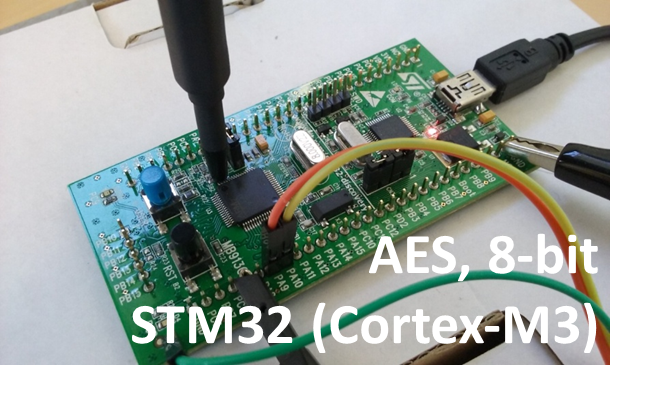
\includegraphics[width=\textwidth,height=0.9\textheight,keepaspectratio]{stm32-EM.png}
%   \end{minipage}
%   \hfill
%     \begin{minipage}{.3\linewidth}
%       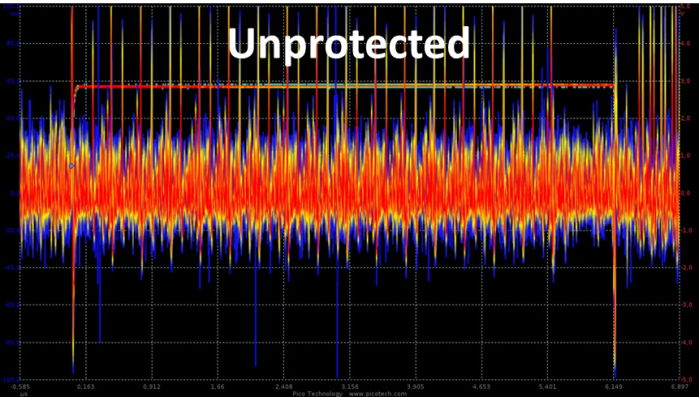
\includegraphics[width=\textwidth,height=0.9\textheight,keepaspectratio]{unprotected.png}
%     \end{minipage}

%     % \textbf{ICI IL Y A DU TRAVAIL!!!!!}
    
% \end{frame}



\section{The Defender's Toolbox}



\begin{frame}
  \frametitle{Defenses - a quick panorama}
  \begin{itemize}
  \item Cryptography: how to encrypt data
  \item Secured communication protocols: how to encrypt data + share keys
  \item Physical shielding: how to protect device from physical alteration
  \item \textbf{ICI il y a du travail}
  \end{itemize}
\end{frame}


% \begin{frame}
%   \frametitle{TODO}

%   \begin{itemize}
%   \item Parler de firewall
%   \item évoquer le fait qu'on va expliquer / comprendre comment marche https. 
%   \item 
%   \end{itemize}
% \end{frame}



\begin{frame}[fragile]
  \frametitle{Definition - Communication Security    \footnote{\url{https://en.wikipedia.org/wiki/Communications_security}}}
  \begin{block}{}
    \begin{center}
      \includegraphics[scale=1]{commSecurity.pdf}
    \end{center}

  \end{block}

  \begin{center}
    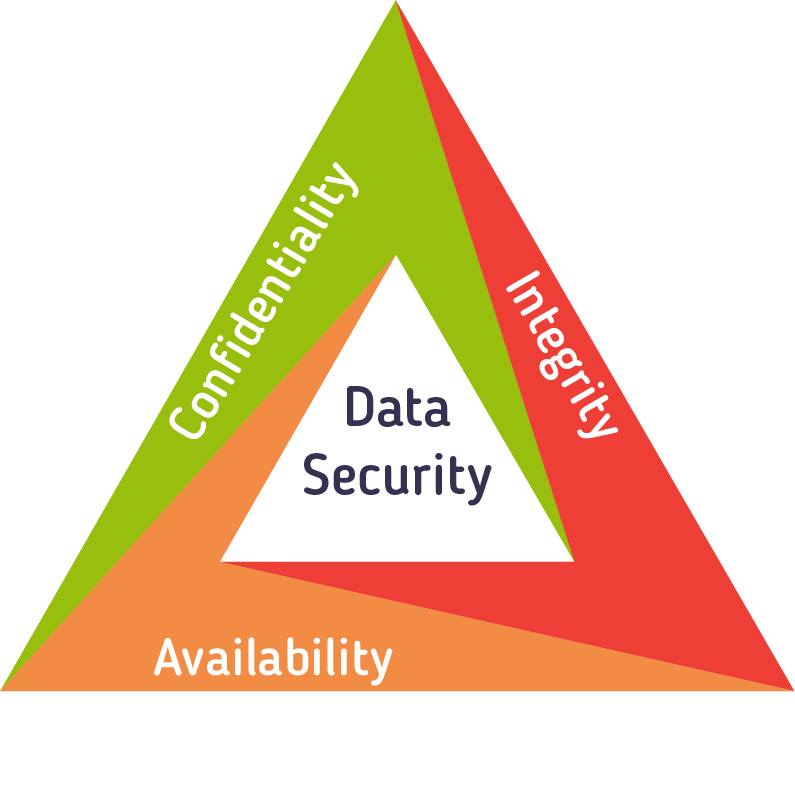
\includegraphics[scale=0.15]{CIA.png}
  \end{center}
  
  
\end{frame}


\begin{frame}
  \frametitle{Cryptology}

  Cryptology, is the science of practice and study of techniques for secure communication in the presence of adversarial behavior.

  \begin{itemize}
  \item \textbf{Cryptography}: Practice and study of techniques for secure communication in the presence of adversarial behavior.
  \item \textbf{Cryptanalysis}: Process of analyzing information systems in order to understand hidden aspects of the systems. 
  \item \textbf{Cryptology = Cryptography + Cryptanalysis}
  \end{itemize}

  In this course, we mainly focus on \textbf{Cryptography}. 
\end{frame}

\section{History}


\begin{frame}
  \frametitle{A brief history of cryptography}

  \begin{itemize}
  \item Keeping message secret has always been a (powerful) men's
    concern ...
  \item  ... but (at least today) it's also of every person's interest. 
  \item ... because there is no ``I got nothing to hide'' 
  \end{itemize}
\end{frame}



\begin{frame}
  \frametitle{History (1) The Skytale}
  \begin{itemize}
  \item Oldest cryprtographic device known (-404 BC)
  \item Write a message on a leather strap
  \item Wrap the strap around a rod with correct diameter
  \item Key = Shape of the rod (diameter, number of sides)
  \end{itemize}

  \begin{center}
    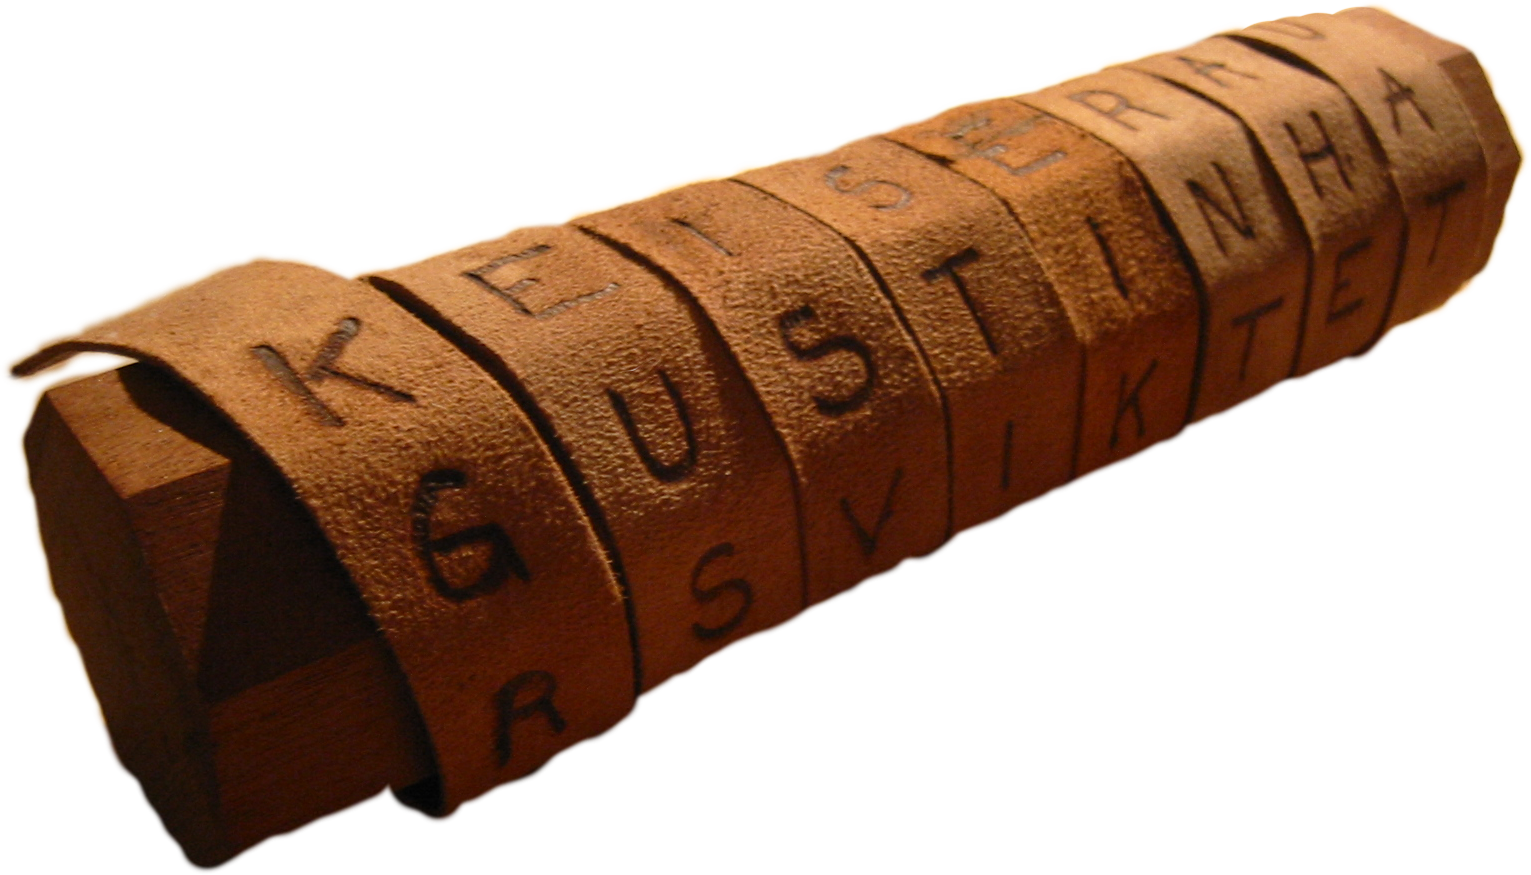
\includegraphics[scale=0.4]{Skytale.png}
  \end{center}
  
\end{frame}


% \begin{frame}
%   \frametitle{TODO}

%   Expliquer d'autres éléments d'histoire, d'autres exemples de chiffrement.

%   Consolider la présentation d'Enigma

%   Finir par l'intro du cours suivant ! 
  
  
% \end{frame}


% \begin{frame}
%   \frametitle{A rajouter dans l'historique}

%   Je repique du cours de François:
%   \begin{itemize}
%   \item La scytale
%   \item Vigenère (mais j'ai pas encore compris)
%   \item Vername (idem)
%   \item Principe de Kerchoffs
%   \item Confusion/Diffusion (Shannon 1949)
%   \end{itemize}
  
% \end{frame}


\begin{frame}
  \frametitle{History (1) Caesar cipher}

  \begin{itemize}
  \item Substitution cipher
  \item Each letter is encoded with its order in the alphabet: A$\rightarrow$0, B$\rightarrow$1, ..., Z$\rightarrow$26
  \item We choose a \textbf{fixed \textit{shift value}} $sh$
  \item To \textbf{encrypt}, each letter $P_i$ in Plaintext is replaced by the corresponding shifted letter:
    \begin{itemize}
    \item[] $\bm{E(P_i) = (P_i + sh) \mbox{ mod } 26}$
    \end{itemize}
  \item To \textbf{decrypt}, each letter $C_i$ in the Ciphertext is converted back with :
    \begin{itemize}
    \item[] $\bm{D(C_i) = (C_i - sh) \mbox{ mod } 26}$ 
    \end{itemize}
  \end{itemize}

  \putat{0.5}{0.75}{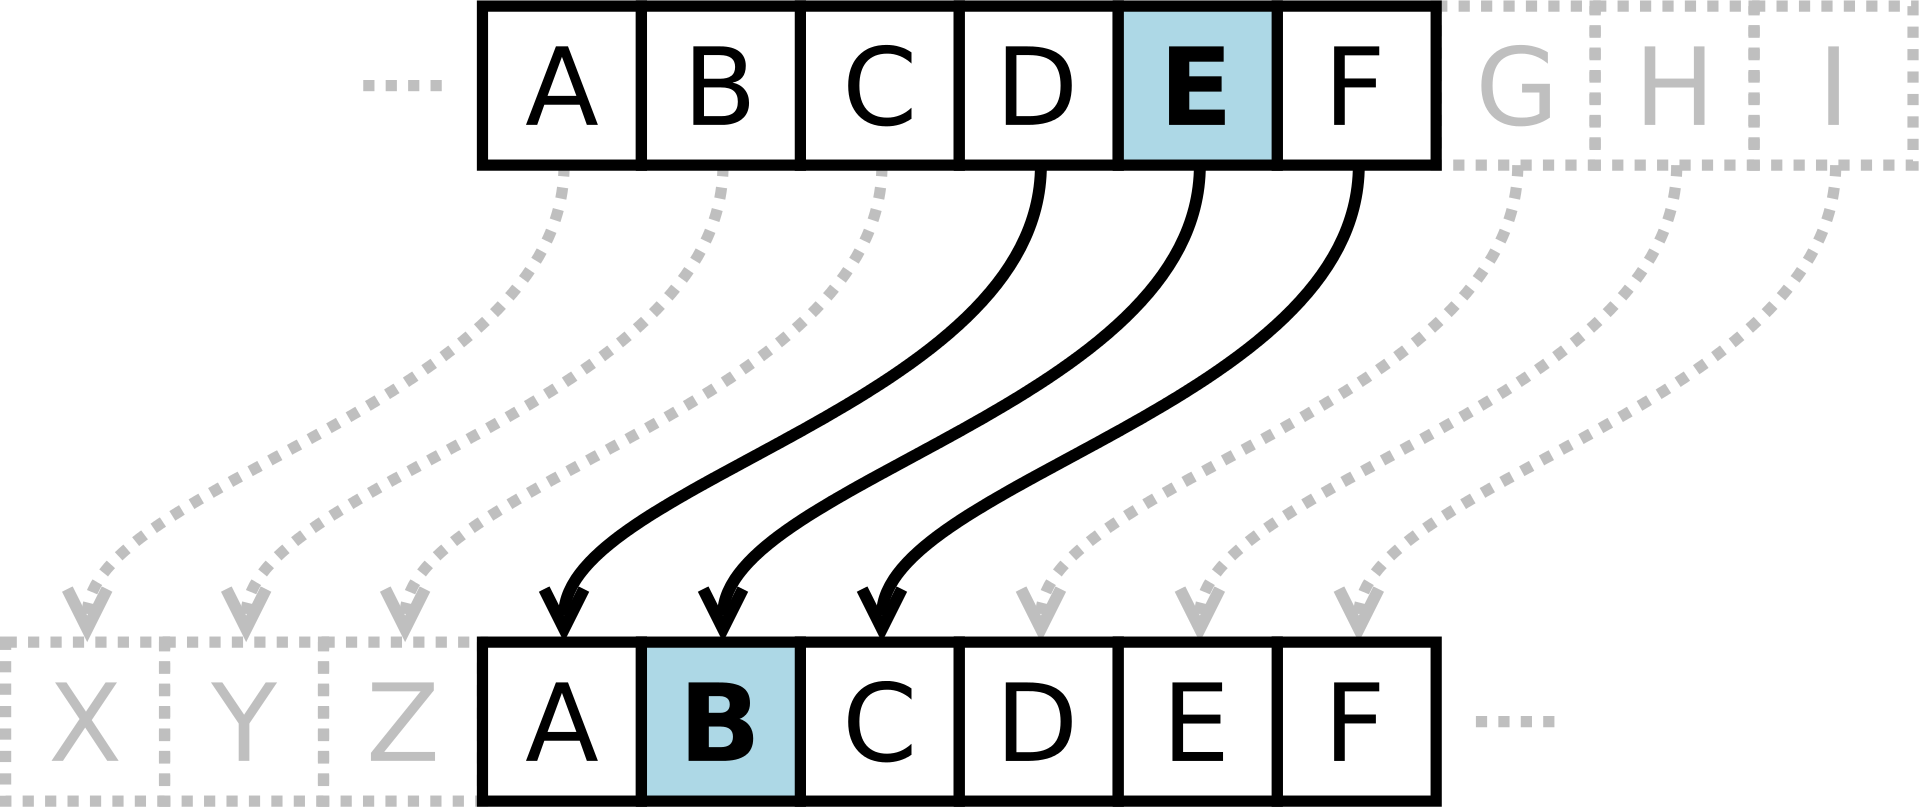
\includegraphics[scale=0.07]{Caesar_cipher_left_shift_of_3.png}}
  
\end{frame}



\begin{frame}
  \frametitle{History (1) Caesar cipher}
  \putat{0.4}{0.7}{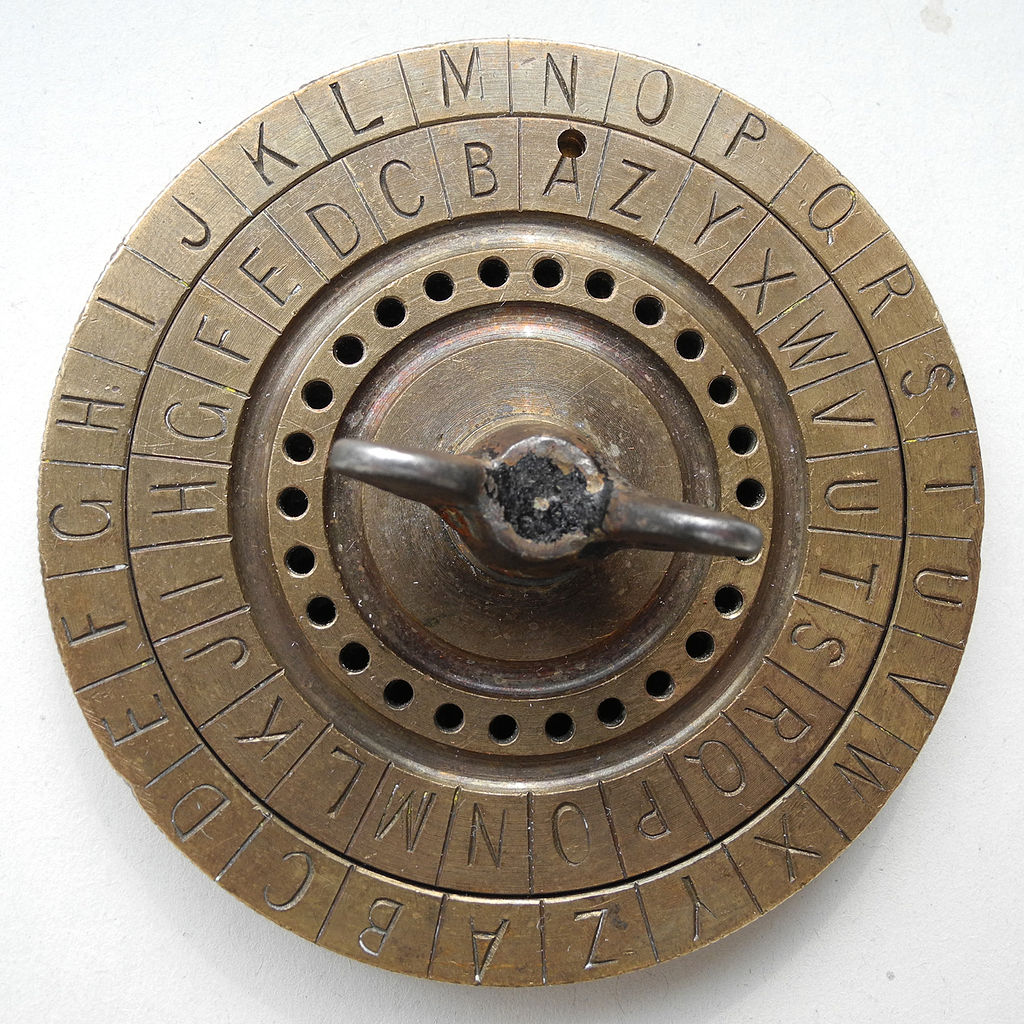
\includegraphics[scale=0.3]{1024px-CipherDisk2000.jpg}}
 
  \begin{itemize}
  \item[\plus] Encryption and decryption are cheap
  \item[\minus] Easy to crack with frequency analysis
  \item[\plus / \minus] Sufficient when no-one around can read :) (in
    particular, what's the difference between a foreign language and
    an encrypted language, if you can't read the first).
  \end{itemize}
\end{frame}


\begin{frame}[fragile]
  \frametitle{General case: Substitution cipher}

  \begin{block}{Principle}
    Replace a letter by another\\
    \verb+ABCDEFGHIJKLMNOPQRSTUVWXYZ+\\
    \verb+AZERTYUIOPQSDFGHJKLMWXCVBN+
  \end{block}
  \begin{block}{Attack}
    \begin{itemize}
    \item Frequency analysis
    \item Each letter in a given language has a specific occurrence frequency
    \item Replace letter with frequency $f$ in the encrypted text by
      letter with frequency $f$ in the original alphabet
  \end{itemize}
  \end{block}

  \begin{center}
    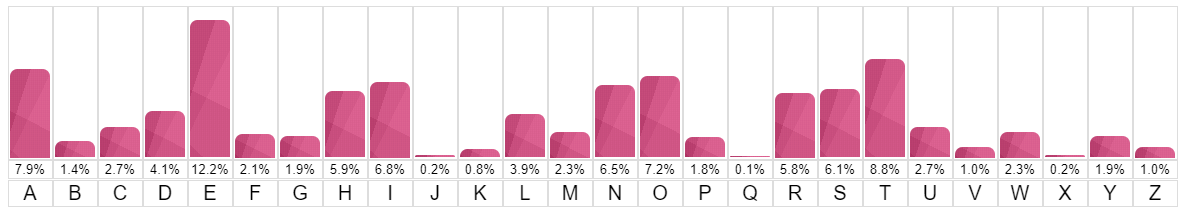
\includegraphics[scale=0.3]{freqChart-EN.png}
  \end{center}
  
\end{frame}


\begin{frame}
  \frametitle{Vigenère cipher (1/3) - Principle}
    \begin{itemize}
    \item Invented XVIth century
    \item Based on a \textbf{Vigenere table 26x26 $VigT$} : \\
      Each line starts by a different letter $\mathcal{L}$ of the
      alphabet and contains the whole alphabet in the usual order,
      starting from $\mathcal{L}$ and looping back from A to Z ....
      \begin{center}
        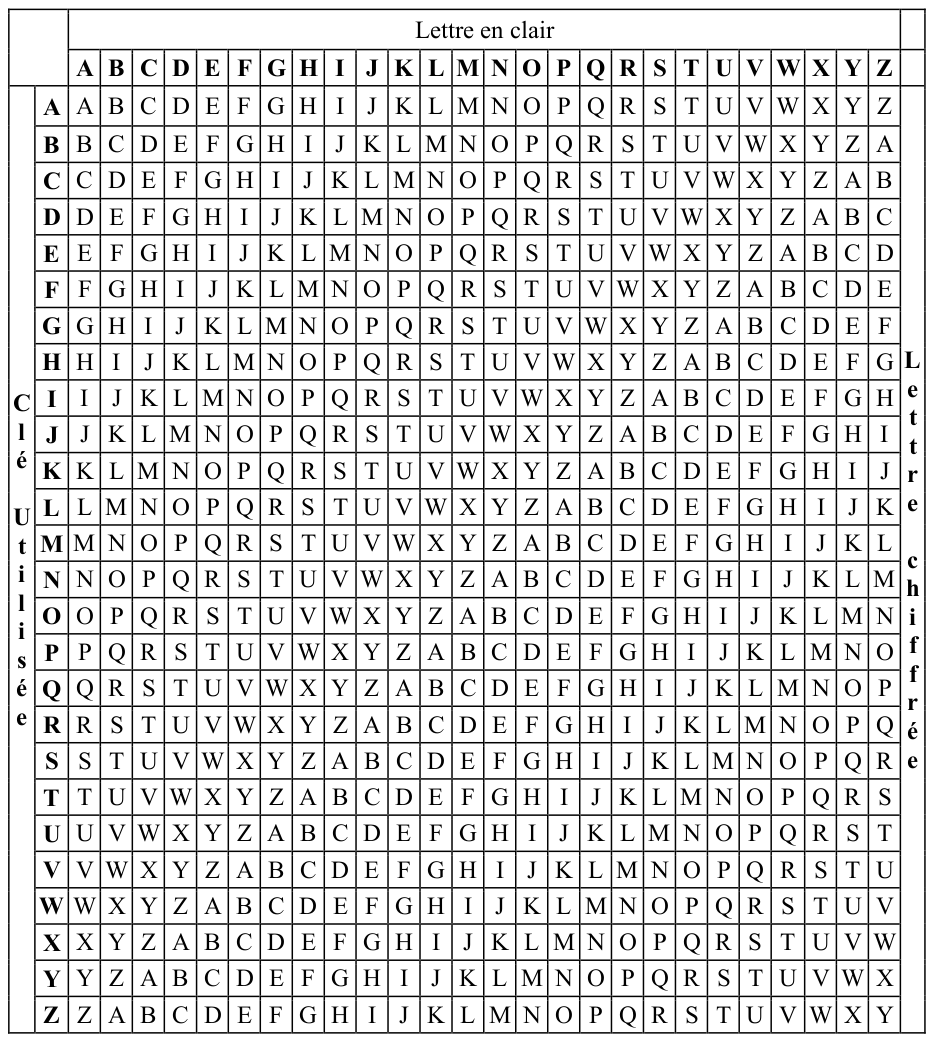
\includegraphics[scale=0.3]{vigenere.png}
      \end{center}
    \end{itemize}
\end{frame}


\begin{frame}
  \frametitle{Vigenère cipher (2/3) - Principle}
  \begin{itemize}
  \item Let's send a message $m$ of length $l(m)$ : \\
    \alert{$m$ = killthekingtonight, $l(m)$ = 18}
    \item Choose a key $k$ of $l(k)$ characters : \\
      \alert{$k$ = HORSE, $l(k)$ = 5}
    \item Repeat the key until you reach $k'$ of length $l(k') = l(m)$ \\
      \alert{$k'$ = HORSEHORSEHORSEHOS}
    \item encoded letter $m_i$ by replacing it by $VigT[k'_i][m_i]$: \\
      \alert{cipher(m,k) = RWCDXOSBARNHFFMNVL}
    \end{itemize}

    \bigskip
    
    Strength: disguise the plaintext's letter frequency to interfere with frequency analysis.
\end{frame}


\begin{frame}
  \frametitle{Vigenère cipher (3/3) - Kasiski's Attack (1863)}
  \begin{itemize}
  \item Some repeated word may be encrypted using the same key letters:\\
%    Key:        ABCDABCDABCDABCDABCDABCDABCD\\
    Ciphertext: \textbf{CSASTP}KVSIQUTGQU\textbf{CSASTP}IUAQJB\\
  \item Distance between repetitions of \textbf{CSASTP} = 16
  \item Assume repeated segments in the ciphertext encode the same plaintext
  \item Key length is 16, 8, 4, 2 or 1 ... 1 and 2 are too simple. 
  \item We know the key starts by A, B, C, D ... Let's try all possible keys.
    
  \item Quite quickly, we find that:\\
    Plaintext:  \textbf{CRYPTO}ISSHORTFOR\textbf{CRYPTO}GRAPHY\\
  \end{itemize}

  \bigskip
  
  The longer the ciphertext, the more accurate the analysis
\end{frame}


\begin{frame}
  \frametitle{One-time pad (1/3)}
  \begin{itemize}
  \item Invented in 1882
  \item Substitution cipher
  \item Choose a \textbf{random key $K$} \alert{at least as long as the plaintext}
  \item To \textbf{encrypt}, each letter $P_i$ in Plaintext is replaced by the corresponding shifted letter:
    \begin{itemize}
    \item[] $\bm{E(P_i) = (P_i + K_i) \mbox{ mod } 26}$
    \end{itemize}
  \item To \textbf{decrypt}, each letter $C_i$ in the Ciphertext is converted back with :
    \begin{itemize}
    \item[] $\bm{D(C_i) = (C_i - K_i) \mbox{ mod } 26}$ 
    \end{itemize} 
  \end{itemize}
  \putat{0.7}{0.6}{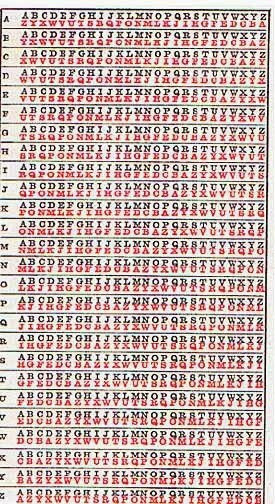
\includegraphics[scale=0.3]{onetimepad.jpg}}
  
\end{frame}


\begin{frame}
  \frametitle{One-time pad  (2/3) - Pros and Cons }

  \begin{itemize}
  \item[\plus] Proven secure
  \item[\plus] Even to frequency analysis
  \item[\plus] Encryption and decryption are cheap
  \item[\minus] Fresh key is needed for every plaintext 
  \item[\minus] Key must be as long as the plaintext 
  \item[\minus] Key must be kept secret
  \item[\minus] Key must not be lost (not by one character)  
  \item[\minus] Key must be truly random 
  \end{itemize}
\end{frame}


\begin{frame}
  \frametitle{One-time pad (3/3) - a long lasting history}
  \begin{itemize}
  \item \textbf{1920}: Weimar Republic Diplomatic Service
  \item around \textbf{1930}: Soviet Union (after breaking of own cryptography by the British)\\
    KGB spies used them until the 1950s and 1960s
  \item during \textbf{WWII}: used in the SIGSALY secure speech system
    for high-level Allied communications
  \item from \textbf{1963}: (after the Cuban Missile Crisis):
    Moscow-Washington-DC hotline used teleprinters
  \item During the \textbf{1970s}: the NSA used them extensively
  \item from \textbf{1988}: The African National Congress to
    communicate between ANC leaders outside South Africa and
    in-country operatives
  \end{itemize}
\end{frame}

  
% \begin{frame}  
%   Un panorama de l'histoire de la sécurité des communications:
%   \begin{itemize}
%   \item Le code de César
%   \item ...
%   \item Le ``one-pad pads'' cipher (dont le problème résiduel considérable est que ça nécessite une clé
%     \begin{itemize}
%     \item Besoin de ``true randomness''
%     \item Peut-être je peux passer du temps à expliquer qu'obtenir du vrai random dans un ordinateur c'set dur. 
%     \item \url{https://www.youtube.com/watch?v=M8Tf9_O7s9c}
%     \end{itemize}
%   \item Enigma et la cryptanalyse de Turing et al
%   \end{itemize}
% \end{frame}


\begin{frame}
  \frametitle{Enigma}
  \putat{0.01}{0.65}{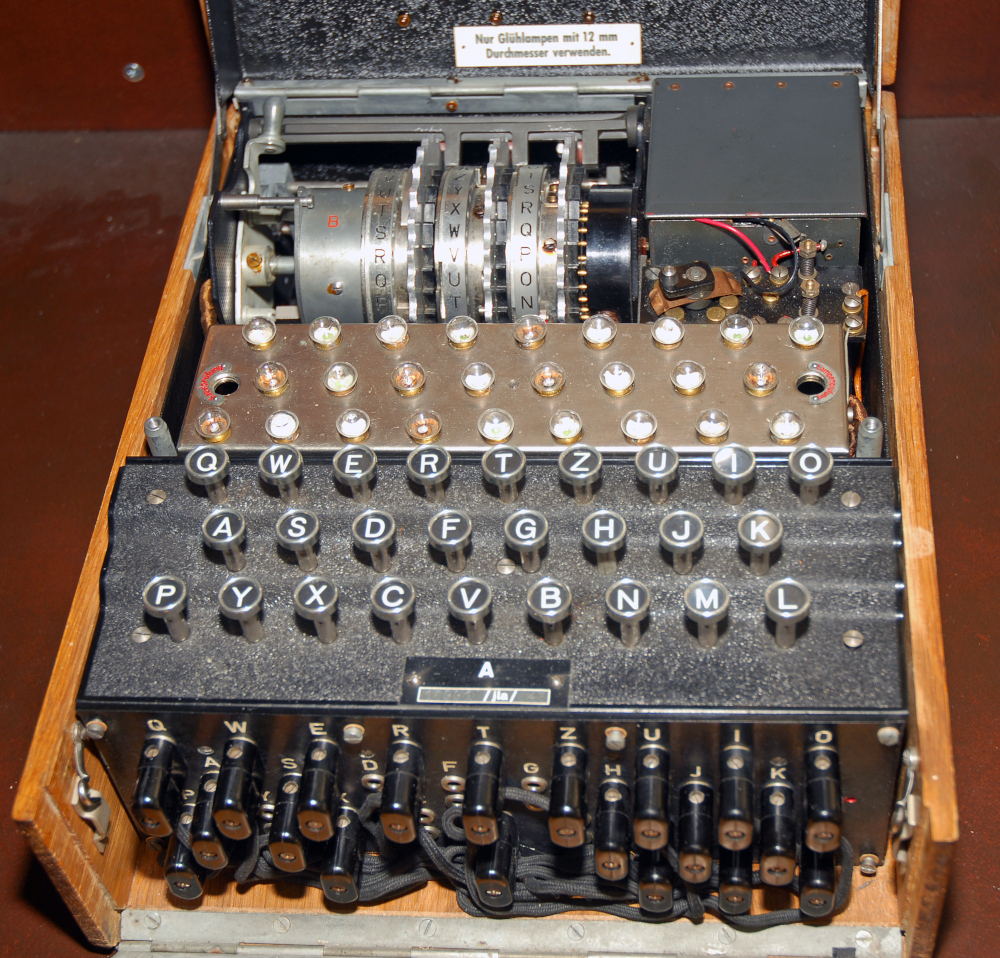
\includegraphics[scale=0.3]{enigma.jpg}}

  \putat{0.25}{0.6}{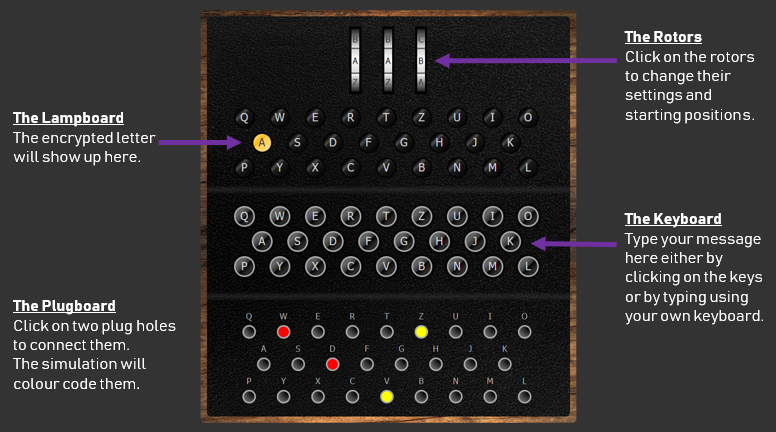
\includegraphics[scale=0.2]{enigma-how-to.png}}

  \vspace{-2cm}
  
  \begin{itemize}
  \item Invented at the end of WWI
  \item Used extensively by Nazi Germany during WWII
  \item First cracked by Polish services during the early 30s ... 
  \item ... then by British-led effort at Bletchley Park, including Alan Turing. 
  \end{itemize}
\end{frame}


\begin{frame}
  \frametitle{Enigma - How does it work?}

  \begin{itemize}
  \item Substitution cipher
  \item Originally patented in 1918
  \end{itemize}

  \begin{center}
    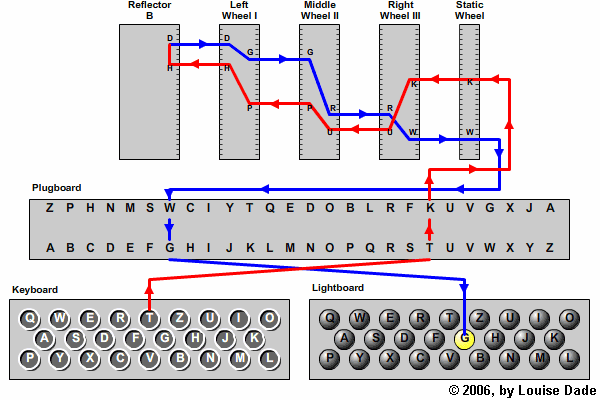
\includegraphics[scale=0.25]{Enigma-wiringdiagram.png}
  \end{center}

  
  \putat{0.75}{0.55}{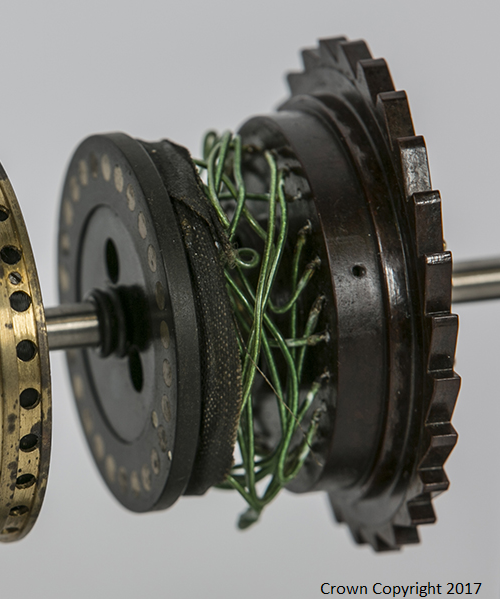
\includegraphics[scale=0.3]{7X5A0921-closeup.png}}

  
  \begin{itemize}
  \item All three wheels are wired differently 
  \item Wheels are initialized to any position
  \item The reflector never wires a letter to itself
  \item Army-grade version :
    \begin{itemize}
    \item Choose 3 wheels amongst a set of 6
    \item Plugboard
    \item Change the initial rotor setting
    \end{itemize}
  \end{itemize}
  
\end{frame}


\begin{frame}
  \frametitle{Enigma - Combinatorial}
  \textbf{Every day}, the machine is reset to a pre-established configuration:
  \begin{itemize}
  \item $60$ Rotors choice (3 or 4 or 5 among 6 possible). 
    % \item $26^3$ Rotors permutation (\texttt{I-V-II} or \texttt{II-III-I} or ...)
  \item  $26^3$Rotors initial letter combination
  \item Plug-board settings: $$\frac{26!}{6!10!2^{10}}$$
  \item The initial setting for a specific day, use a pre-printed
    paper codebook (gives initial configuration)
  \end{itemize}
  % \item \textbf{Every message} contains a rotors position the machine
  %   should be reset to before decrypting the rest of the message.

  \begin{center}
    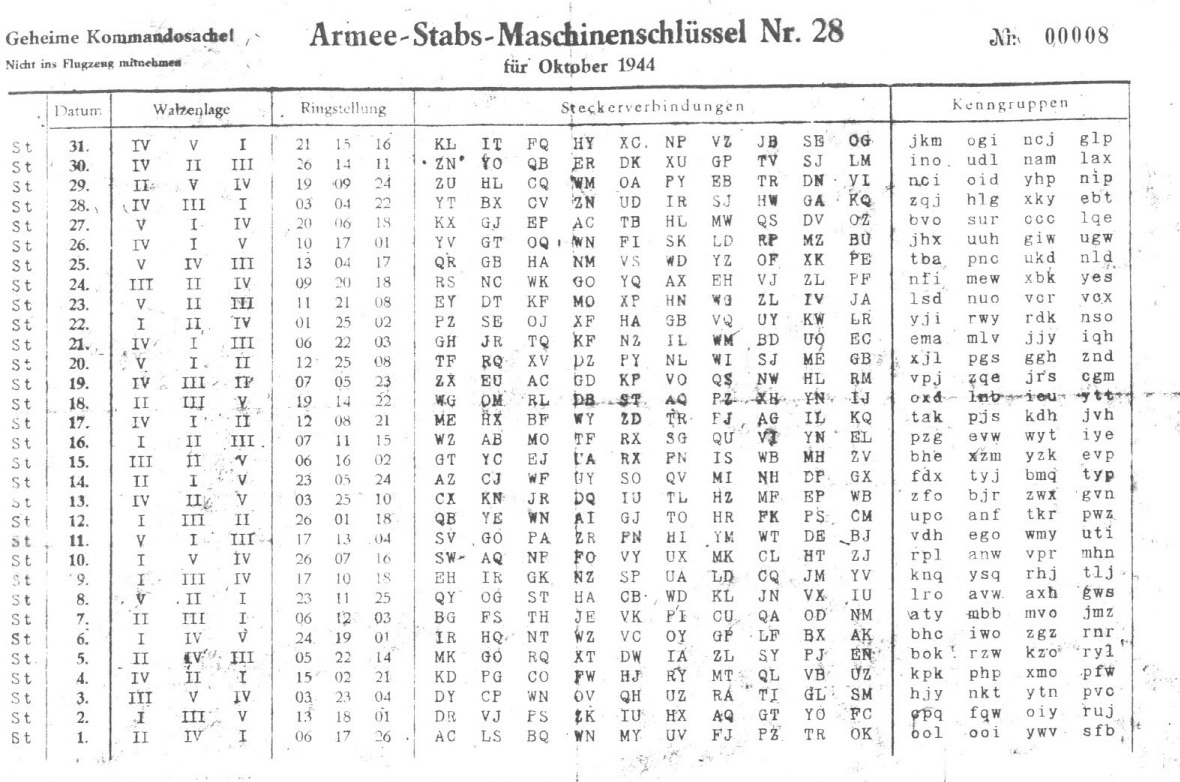
\includegraphics[scale=0.2]{keysheet.jpg}
  \end{center}
  
\end{frame}


\begin{frame}
  \frametitle{Enigma - Breaking the machine}

  \begin{itemize}
  \item To brute-force Enigma is unpractical: > 150 millions millions combinations
  \item A letter is encrypted into a different letter every time ....
  \item ... but never to itself !! \textbf{Main flaw}
  \item Try to guess a word or phrase in a message (and Germans military did use recurring messages, like weather reports)
  \item ...
  \end{itemize}

\end{frame}

\begin{frame} 
  \frametitle{Enigma - breaking the machine}
  \begin{center}
    \only<1>{\includegraphics[scale=0.7,page=1]{exampleEnigma.pdf}}
    \only<2>{\includegraphics[scale=0.7,page=2]{exampleEnigma.pdf}}
    \only<3>{\includegraphics[scale=0.7,page=3]{exampleEnigma.pdf}}
    \only<4>{\includegraphics[scale=0.7,page=4]{exampleEnigma.pdf}}
    \only<5>{\includegraphics[scale=0.7,page=5]{exampleEnigma.pdf}}
  \end{center}
\end{frame}

\begin{frame}[fragile]
  \frametitle{Enigma - Breaking the machine}

  \begin{itemize}
  \item Adding a couple more properties, evict impossible configurations. 
  \item Scan through the remaining combinations using \textbf{the Bombe} : electro-mechanical machine able to ``play'' 36 Enigma equivalent ``in parallel''. 
  \item In the end .... guess the key (wheel starting positions + plug-board) in less than 20minutes per day. 
  \end{itemize}
 
\end{frame}



\begin{frame}
    \frametitle{Enigma}
  \begin{minipage}{0.45\textwidth}
    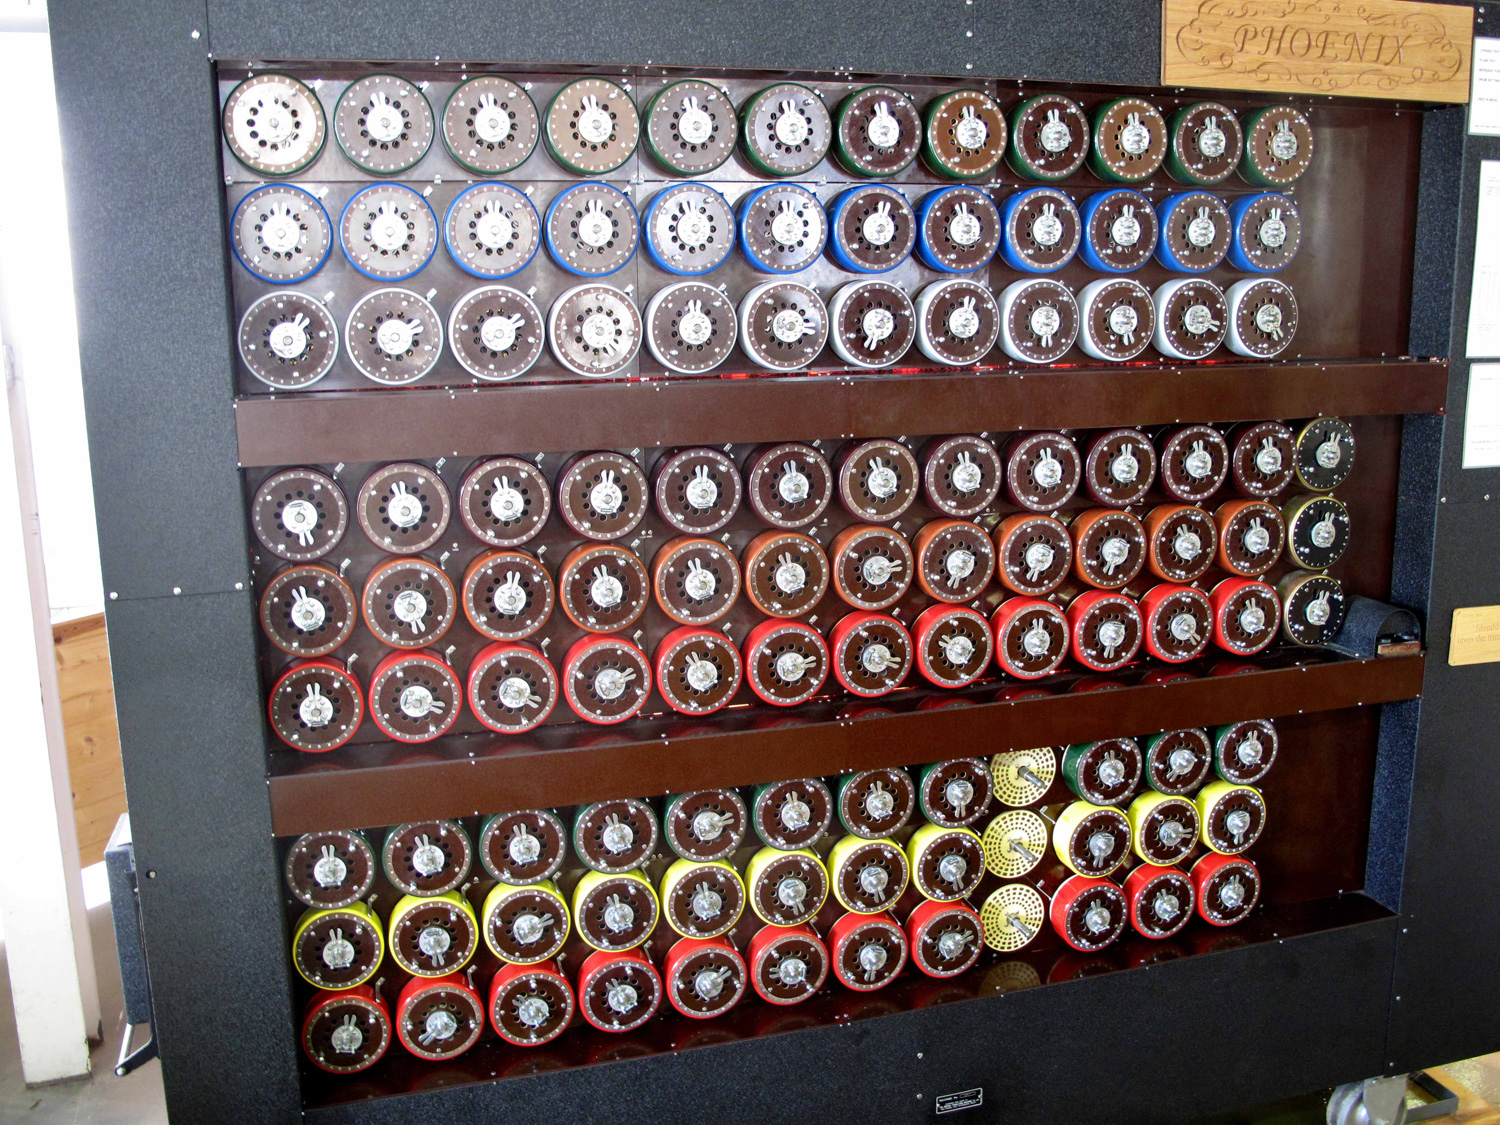
\includegraphics[scale=0.1]{rebuilt-bombe-bletchley-park.jpg}
  \end{minipage}
  \hfill
  \begin{minipage}{0.45\textwidth}
    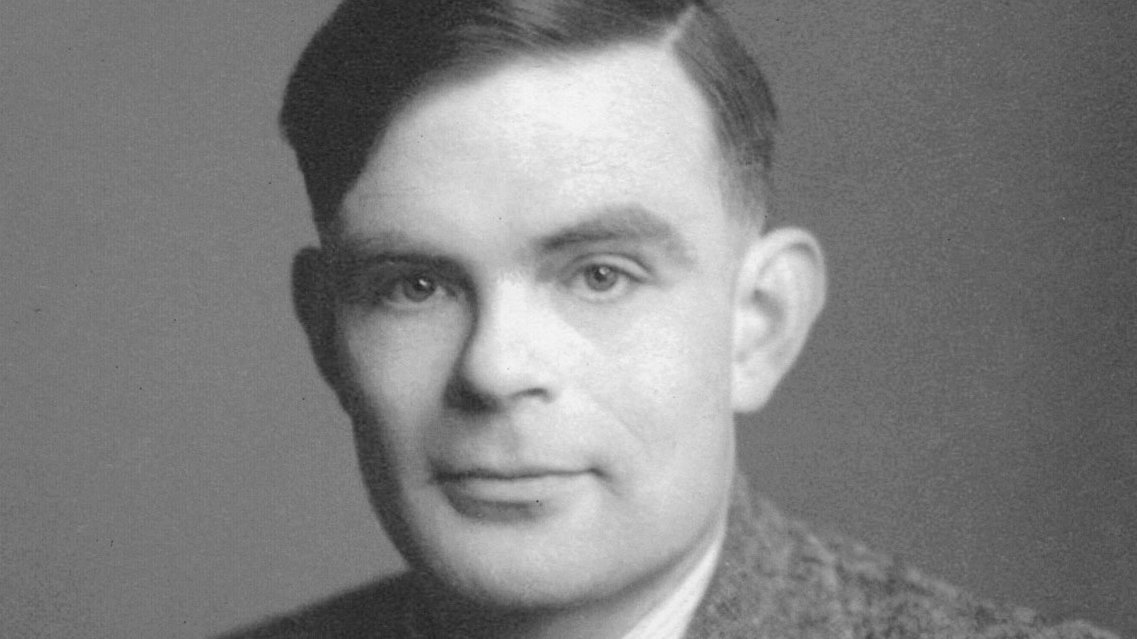
\includegraphics[scale=0.1]{alanTuring.jpg}
  \end{minipage}

  \footnote*{watch \url{https://en.wikipedia.org/wiki/The_Imitation_Game}}
\end{frame}


\begin{frame}
  \frametitle{More Recent history}

  \Wider{\small Symmetric (private-key) cryptography: 
  \begin{itemize}\small 
  \item \textbf{1975} IBM proposes the Data-Encryption Standard
  \item \textbf{1977} DES Adopted as a FIPS standard
  \item \textbf{1994} Differential-linear cryptanalysis of DES is proposed
  \item \textbf{1996} call for DES replacement by NIST
  \item \textbf{1998} Brute-force attack on DES demonstrated feasible
  \item \textbf{2001} AES announced as replacement for DES
  \item \textbf{2023} \textit{At present, there is no known practical attack
      that would allow someone without knowledge of the key to read
      data encrypted by AES when correctly
      implemented. }\footnote{\url{https://en.wikipedia.org/wiki/Advanced_Encryption_Standard}}
  \end{itemize}

  Asymmetric (public-key) cryptography:
  \begin{itemize}\small 
  \item \textbf{1976} Diffie-Hellman key exchange protocol proposed
  \item \textbf{1977} RSA (Rivest-Shavir-Adleman)
  \item \textbf{1985} El-Gamal encryption
  \item \textbf{1985-...} Elliptic-Curve Cryptography
  \end{itemize}}
  
\end{frame}



\begin{frame}
  \frametitle{Course Plan}
  
  \begin{block}{Lectures}
    \begin{itemize}
    \item Symmetric cryptography, Asymmetric cryptography, Key sharing, compromises 
    \item Security protocols: Public-Key Infrastructures, TLS, SSH, HTTPS, Kerberos, VPNs, 
    \end{itemize}
  \end{block}

  \begin{block}{Lab / Paper Sessions}
    \begin{itemize}
    \item Ethical considerations
    \item Applying asymmetric encryption principles
    \item Password storage
    \item Certification and Public-Key Infrastructures
    \item Cryptographic Protocols
    \item Reading survey project
    \end{itemize}
  \end{block}

  All details on \url{https://lmorel-insa.github.io/csc/}
  
\end{frame}





\begin{frame}
  \frametitle{References}
  \begin{itemize}
  \item On exploiting buffer overflow: \url{https://youtu.be/1S0aBV-Waeo}
  \item Turing's Enigma Problem Part 1: \url{https://youtu.be/d2NWPG2gB_A}
  \item Turing's Enigma Problem Part 2: \url{https://youtu.be/kj_7Jc1mS9k}
  \item Some details on the working of the Enigma (with a real machine presented): \url{https://youtu.be/G2_Q9FoD-oQ}
  \item How easy is to crack Enigma today: \url{https://youtu.be/RzWB5jL5RX0}
  \end{itemize}
\end{frame}


\end{document}

  